\documentclass[a4paper,twoside]{stop-article}
\usepackage{tabverb}
\usepackage{lit-style}
\usepackage{psfig}
\usepackage{titlepages}
\usepackage{dir}
\usepackage{hevea}
\newcommand{\lib}{../../lib/stratego}
\renewcommand{\literate}[1][]{\section{#1}}
\usepackage{bgcolor}
\renewcommand{\cuttingunit}{subsection}
\usepackage{stop-onecolumn}
\pagestyle{empty}
\begin{document}
	\input{../intro/arch.ptx}
	
\clearpage% page: 0
	\input{../intro/comp.ptx}
	
\clearpage% page: 1
	$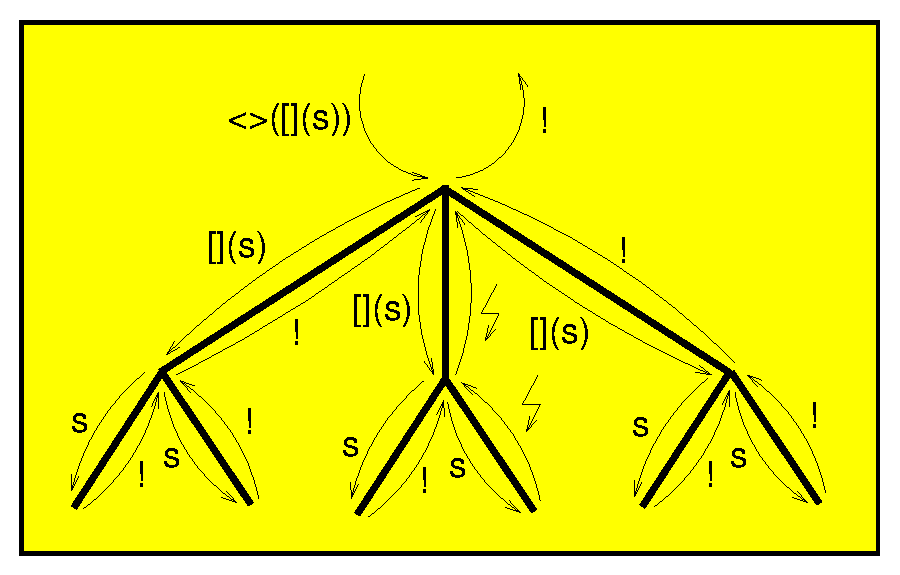
\psfig{file=../intro/treetrans.eps,width=10cm}$
	
\clearpage% page: 2
	\input{../basics/import-graph.ptx}
	
\clearpage% page: 3
	\input{../basics/tree.ptx}
	
\clearpage% page: 4
	\input{../basics/dag.ptx}
	
\clearpage% page: 5
	\input{../basics/transformation.ptx}
	
\clearpage% page: 6
\end{document}
